% Changing book to article will make the footers match on each page,
% rather than alternate every other.
%
% Note that the article class does not have chapters.
\documentclass[letterpaper,10pt,twoside,twocolumn,openany]{book}

% Use babel or polyglossia to automatically redefine macros for terms
% Armor Class, Level, etc...
% Default output is in English; captions are located in lib/dndstring-captions.sty.
% If no captions exist for a language, English will be used.
%1. To load a language with babel:
%	\usepackage[<lang>]{babel}
%2. To load a language with polyglossia:
%	\usepackage{polyglossia}
%	\setdefaultlanguage{<lang>}
\usepackage[english]{babel}
%usepackage[italian]{babel}
% For further options (multilanguage documents, hypenations, language environments...)
% please refer to babel/polyglossia's documentation.

\usepackage[utf8]{inputenc}
\usepackage{lipsum}
\usepackage{listings}

\usepackage{dnd}

\lstset{%
  basicstyle=\ttfamily,
  language=[LaTeX]{TeX},
}

% Start document
\begin{document}

\onecolumn

\begin{center}
Velterra: Sinners Never Sleep
\end{center}

\clearpage

\begin{center}
 
\Huge
The Cast\\
\vspace{20mm}

\large

Michael Williams - Dungeon Master

\vspace{10mm}
\normalsize
\textit{
Stephen Harland - Pilcheur Gamont/Mark O'Synne/Vu Dong/Burnie Cinders \\
Jonathan Mann - Exmerah Sliokzog\\
Richard Pugh - Riphard Obsidian Hardstone\\
Stephen Reddish - Kolo Kozolski Sliokzog\\
Joshua Rodell - Lady Otoria Hearthrust/Gary/Myron  \\
}

\end{center}

\clearpage

\twocolumn

\chapter{Chapter 1: Characters}

\section{Burnie Cinders}




\begin{paperbox}{Example}
  \lipsum[2]
\end{paperbox}



\clearpage


\section{Exmerah Sliokzog}

\begin{center}

\includegraphics[width=80mm]{./img/exme1.png}
\begin{figure}[h]
\end{figure}
\end{center}

\begin{paperbox}{Example}
  \lipsum[2]
\end{paperbox}

\clearpage


\section{Riphard Obsidian Hardstone}

\begin{center}

\includegraphics[width=80mm]{./img/riphard1.jpg}
\begin{figure}[h]
\end{figure}
\end{center}

\begin{paperbox}{Example}
  \lipsum[2]
\end{paperbox}

\clearpage


\section{Kolo Kozolski Sliokzog}

\begin{center}

\includegraphics[width=80mm]{./img/kolo.jpg}
\begin{figure}[h]
\end{figure}
\end{center}

\begin{paperbox}{Example}
  \lipsum[2]
\end{paperbox}

\clearpage


\section{Myron}

\begin{center}
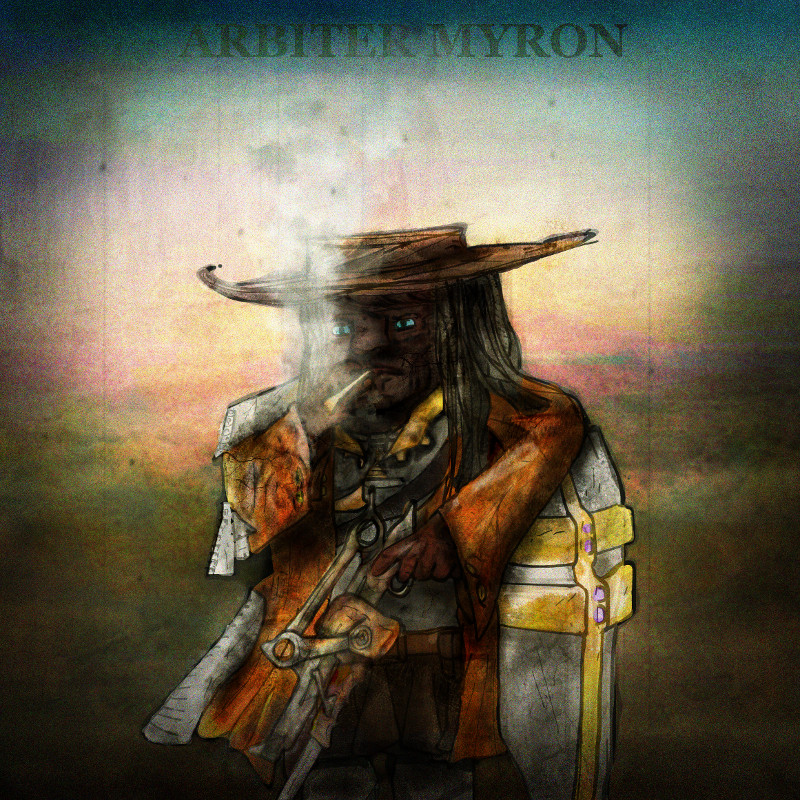
\includegraphics[width=80mm]{./img/myron1.png}
\begin{figure}[h]
\end{figure}
\end{center}

\begin{paperbox}{Example}
  \lipsum[2]
\end{paperbox}

\clearpage





\chapter{Chapter 2: Background}


\clearpage

\chapter{Chapter 3: The Story}

\section{Episode 1: Riphard Begins}

Welcome to the world of Velterra, domain of the Seven, who rule over all from afar through the constant vigilance of the Church.

“In Hope’s Rest, the largest city of the Empire of the Seven, a cloaked man dashes over rooftops, a half-burnt tome tucked under one arm as a group of mercenaries chase him. Abruptly he comes to a dead end, a roof with nowhere to leap to and nowhere to hide. He turns to face his attackers and reaches for his weapons, the book slipping from his grasp as he does so. In a moment of panic he spins to grab for the book, losing his balance and toppling from the roof as the mercenaries swing their blades at his back.”

“In the north, a pair of goblin twins flee the perils of Valkar Varg’s reign, seeking the freedom and new life the south can bring. They are surrounded by brutal tribesmen and vicious axes on all sides, angered by their desertion. As the two goblins look at each other in desperation and anger they nod, the girl raising a long rifle that quivers with electricity, the boy raising a small hunting bow and quickly loosing several arrows. As their enemies close in the bow-user pulls a vial of some mysterious viscous liquid as his twin sister unclips a thrumming round device from her belt. In moments, a huge explosion rips through the area.”

“To the south, a dwarf pastor sits hunched over a tome, scribbling notes. He raises his head as he hears the slow creak of his door, aware that he is expecting no visitors. He stands and turns to see a hulking figure behind him, armoured with a long-barelled gun at his side. The dwarf rests a trembling hand on his holster as a man who should not exist stands before him. Terse words are exchanged, accusations and threats. The dwarf grits his teeth and sets his feet, drawing the pistol at his side as his opponent does the same. From outside, the sound of a single shot being fired can be heard.”

“To the East, a figure wrapped in cloth and strange garments sits quietly in a harbour tavern in Port Averdale, recently arrived on the continent from a long voyage. She sits with an untouched mug of unappealing ale in front of her as three thugs approach the table. They slam down a parchment on the table with a picture and a hefty figure. In a flash she is to her feet, blade drawn and two of the men sliced apart on the ground. She faces the remaining thug who whistles and a stream of men pour into the building from all around. Outnumbered by scores and with a demand the surrender, she chooses the only option she knows. Honour.”

A group of strangers meet up in a featureless, polished stone room, none fully understanding what has brought them there. An elephantine creature (Meredith) beckons them through a mysteriously appearing door into a plush office where a red skinned man wearing a human face mask welcomes them.

The man explains that he is called Lazarus and that the group have all recently died. They have been brought together, here, and given a second chance at life in exchange for carrying out a mission to destroy the Church Upon asking for proof Pilch is shown the full, gory reality of their situation through a window into hell Lazarus explains that the group must obtain the Stone of Anthala from the temple of XXX and our given basic directions. This ancient relic will be the source of future communications with Lazarus and his means of issuing further instructions. They are warned not to gain the attention of the Church.

The group agree to carry out the task and are transported into a cavern, where winter clothes and supplies await them. After some brief introductions Exme opens the cave door to reveal they are in a snowy wilderness The group spend two days walking South (Kolo relieves Pilch of 15 gp during the trip) until they reach the town of Vathos Boundary. During a surprise fight with some wolves the two goblins disappear. Riphard finds that his gun has become faulty but is able to restore it to proper working order with a good clean.

The remaining members enter the town, Pilch in disguise, and go about making inquiries. Riphard and Ontario make a visit to a local smith, not Gerard, who is able to sell bullets and black powder. Onatrio gets the lay of the land, and discovers that the locals are fine with the Church.

The two goblins, desperate to perform their own investigation and disguised as a single person in an overcoat, put Pilch’s money to work inebriating an entire titty bar, whilst loudly exclaiming their adventurous intentions. Otoria witnesses a man being beaten to death in the street.

Several towns folk inform the party about the dreaded masked “tikk-tukks” that lie to the South of the town, these are small bear like creatures with face masks.

The party is reunited in the titty bar. After a brief altercation between Kolo and Pilch concerning some mislocated funds, Exme and Riphard discuss the finer points of owning firearms and Esme is thrilled to get her first real look at a Church gun.

Ontario and Pilchard Meet a hunter named Gerard who gives a brief description of the location of the temple of Anthala lost in the south. Kolo discovers more about what eats people, and gives Pilchs name as a point of contact. Due to the incredible generosity of Pilch’s money, the group are offered free board at the titty bar and take the opportunity to rest up.

The next day they make their way out of town. As they leave, an explosion rips through the local stable, decimating several horses and destroying the building. Riphard is unable to identify the source of the explosion, however Kolo is quick to demonstrate the kindness and superiority of Goblin-folk by using the rest of Pilch’s money to compensate the stable owner for the damage. Along with casting wild aspersions to the gathered crowd as to who might be the culprit, ie only group who has access to black powder (Church).

The group make their way south to the temple

\begin{center}

\includegraphics[width=80mm]{./img/pilch1.jpg}
\begin{figure}[h]
\end{figure}
\end{center}

\clearpage
\section{Episode 2: In the Tiki, Tiki, Tiki, Tiki, Tiki Room}

The year is 6653 CC (Church Calendar). In their search for the Stone of Un'thala, the group set off Southwards from Vathos Boundary following the directions given to them by the hunter, Gerard.

After a day’s travelling the group settle down for the night with Kolo and Pilch taking the first watch. The tension and hatred between the two is palpable and they stare intently at each other. Pilch is briefly distracted, which gives Kolo the chance to disappear. As Pilch desperately searches for his goblin nemesis, Kolo takes the opportunity to attempt to relieve a sleeping Otoria of some of her gold. As he reaches into her pocket Otoria awakes and deals a deadly blow to the goblin, knocking him unconscious.

Otoria throws the bundle of goblin into his tent, awaking his sister in the process, who mistakenly believes it is her turn to perform lookout duties. She sets down opposite Pilch and resumes the goblin-human stare off. Pilch inquires about Exme’s “gun”, but is not prepared for the onslaught of technical information that Exme is only too glad to discuss. The conversation ends with Pilch being none the wiser, embarrassed by his own vast ignorance. When Exme returns to her tent Kolo has vanished.

The group push on towards their goal. After some time they arrive at a large skull shaped ice temple that lies across a perilous looking bridge. Exme refuses to enter without her brother and stubbornly resists the efforts of Riphard to carry her along. Otoria takes charge and heads into the temple.

As the group enter the temple they find themselves in a large spherical chamber, and have their first meeting with the dreaded TikkiTukks™: a race of small bear like creatures with fearsome, culturally insensitive masks. Battle ensues, with the goblins arriving to witness the felling of the final enemy. An investigation of the stone plinth at the centre of the chamber shows that the stone is missing. The goblins remove some masks from the fallen enemies revealing their ghastly faces with sharp, pointed teeth.

The reassembled group head deeper into the temple in search of the stone. Otoria takes a moment to collect some herbs being cultivated by the TikkiTukks™.

Kolo unlocks a locked door, which reveals a room full of small boxes that contain some treasure which the group splits up.** Pilch** attempts to reclaim some of the money that he had "misplaced" in the previous session, shamefully accusing the goblins of thievery. Otoria throws him an azure gem to appease him. As the gold is shared out Riphard warns the goblins: “Next time you want your fair share, join the battle at the right time”.

The goblins attempt to trick another room of TikkiTukks™ by donning masks. Kolo is able to speak in the TikkiTukk™ language. Exme, not knowing of her brothers ability, attempts a bold deception which ultimately backfires when the two are brought to their knees by the devastating attacks from a room full of TikkiTukks™. The group defeat the TikkiTukks™ and enjoy a short rest to recuperate.

As they continue to explore,** Kolo** pulls Exme back, warning her of a strange tangle of silk threads that hang in a corridor. The group is set upon by a giant spider.** Pilch** is able to set fire to the webbing that covers the walls and ceiling, which keeps the spider at bay, but also traps Otoria on the wrong side of the flames as she delivers her swordy brand of justice. After a short struggle the spider explodes in a mass of ichor.

Riphard is having gun troubles.

Continuing on, Riphard activates an ancient trap that fires darts at the group. However, the goblins are not affected since they are of a similar height to the TikkiTukks™; the darts passing harmlessly over them.

The group manage to fight a large room full of TikkiTukks™, slaughtering their leader (who begins the battle with the glorious war cry ‘tikki tukk doumo arigatou tikki tukk’ ) and claiming his glorious mask as their own. Even with their Tikkitactics and Packtics they are no match for the group.

Riphard is still having gun troubles.

The impotent Riphard falls in battle. Kolo kindly revives him whilst pocketing 5 gp, going easy on the man he has no real qualms with yet.

Further battles ensue. Otaria falls. In a desperate attempt to revive her Exme accidentally punches her in the face, pushing her one step closer to death. Kolo looks on in dismay. Riphard is able to revive her, and the two share a tender moment as he lays his hands on her for “a little too long”.

Freshly rested the group find a corridor of doors. In full synchronisation, the crew knock down 4 doors only to find, to Kolo’s dismay, more doors inside: “More DOORS. TRICKSY, TRICKSY!!”

Riphard takes a moment to explore and comes across a fresh water well. He drinks from it and feels the benefits of its cool water, but already feeling 100% despite the recent battles, does not fully appreciate the benefits the refreshing beverage provides, and so does not share this wisdom with the group.

The noise of the group knocking/cutting in half doors causes the TikkiTukks™ to bear down upon them.

Riphard is still still having gun troubles. Exasperated, he makes one last effort and is finally rewarded for his patience and persistence, destroying what once was a young TikkiTukk's™ face in one well placed and devastating shot.

The group leave one TikkiTukk™ alive to interrogate and help them locate the stone. Whilst passed out, the TikkiTukk™ is tied up and hung upside down. The two goblins don their masks and get ready to intimidate him. Kolo leads the interrogation. The TikkiTukk™ is keen not to die and quickly reveals that the stone is held in the chief’s room. In exchange for the location of the stone of Un'thala, Kolo promises the TikkiTukk™ that he can be the new TikkiTukk™ chief.** Pilch** is also offered as a “sweetener”.

Kolo is keen to take the prisoner along, but Otoria cryptically states that she is to “have her way with him”. Pilch, greedy for the prisoner’s vitality through his curse attempts to end its life. Otoria is able to block the first blow, but misses the second, which slices open the TikkiTukk’s™ throat. In a cool rage Otoria pins Pilch up against the wall with her large sword and warns him: “I have to work with you, we have shared goals. But you will not do that again”. Pilch is filled with an intense terror at these words.

The group collect themselves and prepare to head to the chief’s lair to collect their prize

\begin{center}

\includegraphics[width=80mm]{./img/kolo2.png}
\begin{figure}[h]
\end{figure}
\end{center}

\clearpage


\section{Episode 3: The Horse Whisperer}

The group begin in the bedroooms of the Tiki Tuks after the brutal, and controversial, murder of the "friendly" Tiki Tuk by Philo.

The goblins, unimpressed with this behaviour and sympathetic to the Tiki Tuks, head towards the treasure room.

A brief encounter in the water well room see Riphard unsuccessfully attempt to hold Pilch’s head underwater for more details on his violent nature, but Pilch is able to bat him away, swinging his head up in a glorious little mermaid inspired fashion. When asked why he killed the Tiki Tuk, Pilch looks genuinely conflicted.

Riphard wanders down an unknown corridor, much to Kolo's chagrin. Riphard explains that while Kolo just wants to find the treasure they know about, Riphard wants to find "the treasure that we don't know about”. Riphard is rewarded for his inquisitiveness by finding a stable full of boar and two more Tiki Tuks. Kolo is able to deescalate any possible fight using his language/diplomatic skills, thinking quickly on his feet about an alibi where he is actually visiting his uncle. The goblins laugh at the success of their favourite trick.

Riphard discovers another large corridor, this one lined with spiked walls and a mossy floor. Exme is able to discern that this used to be a booby-trapped room, however, it has long since fallen into disrepair. However, she does notice the strange fungus growing on the floor and harvests as much as she can along with her brother. Riphard is asked to help, but stubbornly refuses, not being one to do groundwork for such lowly creatures as goblins. Pilch is asked and curiously finds himself accepting the instructions.

The goblins head to the chief’s rooms. Exme discovers "nothing at all" in a room that she inspects, whilst Kolo recovers a strange, smooth, and intricately engraved stone under a pile of furs in the chief’s bedroom.

For some reason Pilch decides to argue that this might not be the fancy stone we have been sent here to find. Riphard queries just how many fancy looking stones Pilch thinks Tiki Tuks will have. Exme fumbles through her bag for a while, eventually pulling out a strange device which she passes over the stone. It delivers a small printed out piece of tape in Goblinese which she eyes before confirming that it is indeed the stone of Un’thala. Otoria is not surprised as she feels that most normal stones would not have received such careful treatment and preparation. The goblins inform the group that it is time to sleep, but the rest of the group resist the idea.

The group take some food from the stores, but are urged by Kolo to leave some for the Tiki Tuks. Kolo also leaves a message saying “nice to see you uncle”.

Pilch is racist.

The group travel for half a day, back towards Vathos Boundary, Exme noticeably struggling with her large and heavy bag. The group set up camp. Exme disappears for a short while and returns with herbs that she starts combining with the fungus in a small pestle and mortar. The entire group finds themselves falling asleep.

During their sleep they share a common dream in which Lazarus speaks to them and congratulates them on their progress so far. He lays out the next challenge, which is to head north to Hope’s Rest. He reveals Pilch perhaps has the closest connection to his kind. He instructs the group that they are to set up base in this liberal township, and will require money and transport to further their interests. The dream fades around the chuckles of Meredith.

The non-goblins in the group feel weary and drained.** Pilch** deduces that they may be suffering from Zukor’s Rot as a result of being shot with ancient darts in the Temple of Un'thala.

Exme hands Pilch a single packet of grey paste. She thanks him for his help in gathering the fungus, but berates him for his treatment of the murdered Tiki Tuk.

The group travel back to town and Otoria begins making inquiries concerning the exploding stable. Kolo and Exme mysteriously disappear. It is revealed that on top of this disaster, the town is now suffering from a spate of horse robberies, including those that led a caravan which is rumoured to be travelling to the north.

The group visit Black Smith the blacksmith where Kolo, mysteriously reappearing, requests new daggers. Exme, also mysteriously reappearing, attempts to hire the workshop to complete a project. Smith is initially dismissive, however his mind is changed rapidly when offered an ornate, solid gold necklace in return. The goblins begin their work, Exme concentrating hard on her work, and Kolo jumping maniacally on the bellows and hitting things with a hammer. The remaining members head to the titty bar.

Pilch tries some new, innovative ways of begging - he attempts hawks the Tiki masks as blood money, and gets a free drink from other alt-right extremists, but is told to sell the masks to the captain of the guard.

Riphard follows the blacksmith home and, once he has gone to bed, breaks into the man’s home and steals the necklace back. The rest of the group is unaware of this.

The group meet up in the morning and Riphard inquires where to fence sell "totally legitimate jewelry" in the town. He is directed to a jewelry shop where he is given a reduced price for the necklace. Shops have to make a profit, so that is completely normal practice and not a reflection on Riphard's bargaining skills.

The group head to the city guards offices to inquire about potential jobs and the stable mystery, that isn’t really that much of a mystery when you think about it because it was probably certainly a black powder gang or church related jobby.

They meet the half orc captain of the guard Urnok and his troll “friend?” Gumshoe. The group discusses local issues and learns more about how they may secure passage to the North.Kolo is a good detective gabrin. Riphard assures people he is a real pastor. Pilch sells 6 Tikki Tuk masks.

The following jobs are highlighted:

    Giant boar - Farmsteads in the North offering 50 gp to kill it.
    “Jennie’s girls” - Ex-whores who turned to crime after their profession was officially outlawed. Spread like herpes through the empire and can most likely be found to the north. Their leader is a woman called May or “some bitch called May”. The group is told t'arrest her, May.
    The SRA - Small Rights Activists. A collection of, mainly, gnomes and halflings who perform terrorists acts in their most-likely justified quest for improving the rights of smaller folk. Leader is Razzle Backshine, a gnome with a penchant for exploding things in people’s faces. Also spread out through empire.
    Diego Escabar and his Merry Men - A charming half elf who claims to steal from the rich and give to the poor, but doesn’t actually do the key last bit. Likely located in woodlands nearby. This is a local group.

Jobs are paid at a going rate of 5gp per severed left ear. Riphard wants to provide scalps, but is informed by Urnok that scalps are too easy to forge. Riphard accepts this explanation, explaining to the group that ears have a unique print, like fingers, which can be compared to the ear-print database the chief almost certainly keeps for this very purpose.

The gabrins try to turn Pilch in to the guards as Diego, but are unsuccessful. Riphard wonders whether Diego's men would live in a sort-of ghetto, a "robbing hood" if you will.

Pilch points out that it may be useful to try and recruit these groups, or at least align their interests with our own, and work together against the church.

Kolo asks Pilch if he has had sex. He replies that he totally has.

Riphard does not want to arouse suspicion and tries to persuade the group to let him visit the local pastor by himself. After some initial reservations the group allow him several minutes alone before they also insists on seeing the pastor themselves for no discernible reason or purpose.

Riphard's meeting with the pastor gets off to a tense start. “Are you here to help me?”. “Quite the opposite”. “You’re here to hinder me?”. Riphard questions the pastor on "the inquisition", but the pastor bats away his inquiries as mere tall tales. Riphard attempts to show the pastor proof of the inquisition by showing him the fatal wound he received that sent him to hell, but upon lifting his shirt finds his body shows no signs of trauma at all. The pastor tells Riphard he should ignore these scare stories. Riphard replies that in fact it is the pastor who should not ignore the warning signs. The rest of the group is unaware of this.

Riphard storms out and walks past the group without a word, looking very pissed off. The group take this as a sign to enter themselves.

Otoria and Pilch question the pastor, who has suddenly developed a tremendous stutter for some reason, and learn some things about how the Church operates, predominantly linked to their communication channels.

Riphard looks at boobs, too cheap pious to pay for a touch.

The group end up in the titty bar where Kolo is able to charm/seduce the busty barkeeper into revealing that she used to know May, back in the day. She reveals that May can be expected to be found to the east of the First River. The lady, flushed with lust towards the sweet-talking Kolo, retires to a back room to cool down. Kolo mysteriously disappears again.

The group spend a final night in the titty bar before setting off on their next adventure. As they sleep Lazarus visits them again to tell them that now they are in possession of the stone, some members may find themselves more attuned to any pre-existing magical conditions, but that this shouldn't affect their premiums.

\begin{center}
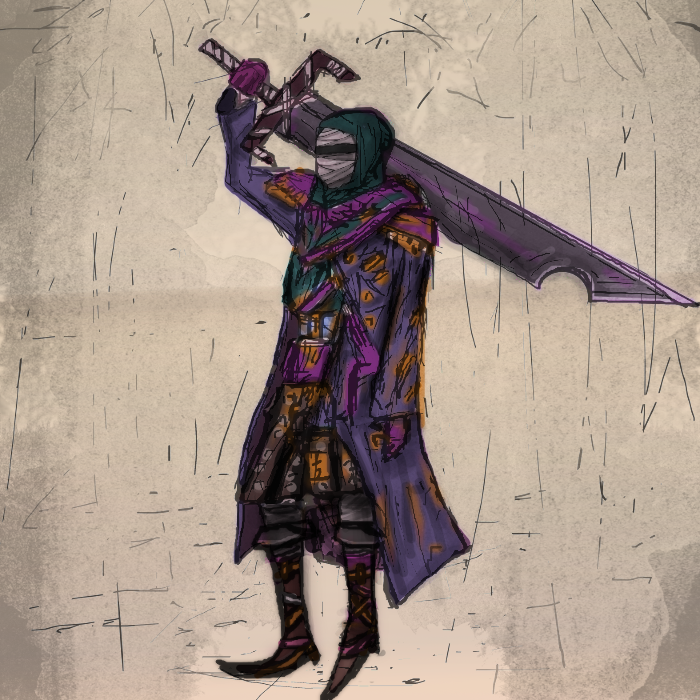
\includegraphics[width=80mm]{./img/otoria1.png}
\begin{figure}[h]
\end{figure}
\end{center}

\clearpage
\section{Episode 4: Whores or Boars?}

Returning to Vathos Boundary, Otoria and her assorted friends are seeking passage North, and have been given a list of gangs that may have stolen all the horses.

They wake up in Marcey’s and try to decide how to proceed.

Otoria wants to infiltrate the Heights Rights lot. Gabrins wants to hassle the Fancy Men.

Riphard sits in the pub, the Gabrins run off.

Riphard wants to walk 6 months instead of finding any horses. He sits in the pub by himself to try and achieve this.

Gabrins and Otoria else goes to see the Blacksmith who’s real sad. Apparently his necklace has got stolen. Otoria wants to find it. They go off to the Blacksmith’s house and look for clues.

Pilch and Riphard bond.

CSI:Vathos ensues at Black Smith’s house. Apparently the necklace was stolen by one non-small person. The fidelity of the blacksmith remains in question.

Kolo looks for criminals to ask questions.

Riphard is pissed. It’s, like, 12:30. Pilch leaves him to his own demons and goes to wander the streets aimlessly.Then, all of a sudden he discovers something important.

Meanwhile, or earlier or something, Otoria talks to the police man and he suggests she checks the local jewelers, so see if whoever stole it tried to sell it. She says she’ll have a look.

Gabrins go into the Mos Eisley Cantena, and talk to a big orc man. Kolo tries to be tough, but is absolutely not that and gets thrown around and nearly thrown out. Then Esme gets involved and is intimidating as fuck. She tries to get the orc man to play cards to win information about the Fancy Man, but that doesn’t work. There’s all sorts of back and forth.

Then, a “Fancy” Woman appears (not a “Fancy Woman”). She offers to help the Gabrins if they come to their hideout. They say they’re going to gather everyone up and head out with her.

Pilchard found an old man. He talks to him about how things aren’t as good as they used to be. There’s also not as young a man. Their names are Casper and Germaine. They are woodsmen. He scares them by being a crazy person. There is no inquisition. He asks them if they know any benders. Pilch is a weirdo.

Otoria finds the jeweler, and the necklace, and the truth.

Riphard is pissed. Then he’s outside in the alley, propped up against the bins, with Otoria trying to kill him, and then Gabrins trying to steal his money. The Gabrins want to keep him alive, but Riphard himself doesn’t seem to have as much interest in that and tries to shoot Kolo. He misses, and Pilch turns up. Riphard tries to run and is instantly struck down. It’s tragic.

Otoria starts dragging him to the police station. Half way there she’s convinced to take him the blacksmith’s instead.

The blacksmith convinces Otoria not to take Riphard to the police, when the group tell him everything, because he would be killed by the church, attracting a lot of attention. Otoria wanted to cut him into little bits, so she’s not super happy about him getting away scot free.

The group give the blacksmith a shit ton of money, then go back to the pub. Riphard sleeps his pain away.

Gabrins stack up inside a coat, and everyone goes into the alley to meet the lady.

The lady is totally fooled by the Gabrins in the coat, for real. She insists on the group helping her or some shit before she tells them where the fancy men are.

The group head North, out of town, to Whorecity. Then west, then through some hills, then some hillocks. Then there’s a camp. It’s a little bit secret. Otoria and the lady (who’s called Delilah) get on like a horse on fire (like what happened in the stables that time).

WELCOME TO WHORECITY!

The group get taken to the Queen Whore, Mae. They brag about their wealth, insult Mae’s fashion sense and then finally get round to actually talking about why they’re there.

Djago and Mae don’t seem like besties, but Delilah jokes that they are. What’s up with that?

Exme wants to know what whoring is.

Otoria wants to know where the horses are. Mae implies, but does not say, that she knows where they are, but says they need to do work for her first.

Kolo makes a deal. No one’s quite sure what it is.

Apparently the whores buys their boots in bulk. They’re damn fine boots. We should get some.

Mae admits the Fancy Men have all the horses, and says she’ll tell them where to find the Heights Rights lot, so they can kill them, and then she’ll tell them we’re the Fancy Men are, so that they can kill them.

Otoria tells Mae not to tell anyone they’re there. Esme tells Mae that they’re terrorists planning to take down the state.

Everything seems fine.

Mae has work to plan.

The gang manage to get two horses, and squeeze on to the back of them.

Riphard gets hit on

They ride horses to Razzle’s house. Razzle is king of the Height Rights. This is his house.

Gabrins are going to go in first, like they’re HeightRightsers. They’re going to see if they can find Razzle, and then come back and do some Strats and Tats.

Gabrins enter HeightRightsManor.

There’s a fucking hobbit.

He’s going to fucking whistle like a bellend.

The Gabrins shout at him and introduce themselves, to get ahead of the scandal.

The fucking hobbit’s called Nickles.

“Big rights for small people”, says Esme.

The Gabrins tell Nickles that they’ve been persecuted for being little. Kolo has terrible flashbacks to the Cantena. This pleases Nickles and they get taken inside.

I can’t really see what’s going on any more.

There’s a sleeping area and some stairs.

Here’s Razzle. He’s a gnome. He’s got a big bag of fireworks. He’s stressful to listen to.

He’s a little leprechaun gangsta, see.

He wants to burn Djago down, see.

Esme tells everyone about wanting to bring down the church again. Razzle wants to kill humans indiscriminately. It’s a debate for the ages. Only Razzle can use the boomstick.

Esme’s, like “please”. Razzle’s like, “NO”.

Esme offers information about booms, in return for… a thing… or… anything. Hundreds of short people will die, but I think that’s the plan. I really don’t understand. It definitely sounds like they’re not going to kill this guy.

Razzle wants Gabrins to kill whores.

Razzle wants to be quiet and small. He’s failing at half of that.

Kolo wants to pick up part time job killing humans, Esme thinks they should focus on taking down church, so that they can kill even more humans.

Gabrins suggest Razzle should come with them on mission to kill whores. Razzle says no. He sends his best men, though.

The Gabrins and the best men go out into the woods, where the Bargins plan to kill them. Otoria and Pilch talk about when to kill everyone.

They eventually decide to wait until everyone’s asleep.

In the woods, everyone’s asleep. Time to die.

Pilch tries to back out of this whole thing, trying to get the Whores and Height Right’s to be friends.

Otoria wants to cut off their tongues and hands.

Esme is spread the gospel of The One, trying to convert the Best Men. Esme and the Best Man (who’s a woman) take a minute and pray to The One.

Everyone else is hanging out in the bushes.

Everyone suddenly doesn’t want to kill them any more. They feel really bad for the small people, but then they kill them anyway.

There’s a brutal massacre.

Everyone decides that they’re going to kill Razzle, but that they want the small people to be free and happy under a new ruler.

Everyone gets back to the cave and prepare for shit to go down.

TO BE CONTINUED...



\clearpage
\section{Episode 5: Pitter Patter of Tiny Bears}

[The following pages are torn from a larger volume, and hastily rebound with string - One corner is singed implying someone attempted to burn this or the entire volume.
The writing is in a quick, hurried, but practiced hand, and the type-face changes occasionally as though the writer grew bored of their style]
Codenames as follows...
- SH - Shadow Hound - Yours truly
- RP - Righteously Pissed - the drunken dwarf
- JR - Jilted Royal - the foreign lady
- SR - Shifty Rogue - the thieving goblin
- JM - Joyful Mechanic - the inventive goblin
So we’re in a cave, and just slaughtered a small number of small folk to whom we hope to ally. Great.
SR has initiated a plan to take over the small-peeps by killing Razzle, SH says we should try and discredit the small folks leader (Razzle) - Seems that the goblins and Dwarf are going to go in and try to convince everyone else that he’s gone rogue and isn’t part of the organisation anymore.
I’m loath to split the party, but the tiny bigots (...small-ots?) probably won’t like me or JR walking in - maybe we can be guards or sympathisers?
Anyway, I do the honorable thing of burning the bodies (and taking 5 ears), and then forging a document for RP -
"Razzle is accused of collusion against the SRA with his Ofecal Cherch Buziness."
We stop outside, and finalise the plan - is as above, but the goblins will go in shortly afterwards to make it seem they were (recently) ambushed.
RP Successfully enters the camp, thanks to the forged letter. The goblins sneak in after. RP manages to get found as an imposter, despite the letter. He did not know the secret Nichols handshake.
A fight breaks out between RP and 3 members of the SRA - but he’s quickly subdued.
Everyone decides to scapegoat RP as a church-worker, still to discredit Razzle. Goblins sneak in.
SRA becomes SRM - suddenly, because RP.
Goblins come in, pretending to be injured - leant huge credence by my amazing disguising. Two of the SRA fall for it.
RP gets blown up. Probably. Razzle likes bombs. “No dwarfy… I expect you to die!”
RP starts whipping people. He gets knocked out.
Team gobbo and 2 of the SRA run in. One gets blown up, the rest like Razzle more for this.
JR is very noisy, it messes up our stealthiness.
SH becomes a rock.
I get RP back up by punching him, and then dance like my life depends on it (which it did).
RP is then useful by disarming Razzle.
Razzle Shanks me, but the shadows protect.
The JM Blows off Razzles head.
SH, RP and JR (who had been doing pull-ups the whole time) leave.
The goblins appoint “Buttons” as the new leader of (this faction) of the SRA.
There's maybe 4 SRA left.
They also loot: Signet ring (with stampy well) 10 rockets 10gp
Papers - Bits of communication, Old Plans, Promotional Material, rambling letters,
I’m not happy about this.
We rest up.
Kolo and Otario have a heart to heart.
We all go to see Mae. JR takes point in the conversation. It’s interesting. Mae and Delilah plan with us to go kill fancy-pants.
I’m on a horse.
Mae gives us 3 people to go take on Fancy-Pants, Diago. One is an Battle-axe barbarian type, others a Crossbow-marksman, as is Delilah.
JR and JM also get fancy “dutty ho” boots.
On the way (to Diago) we encounter a man that tells us about the giant boar. Delilah flirts with RP for some reason.
JR - with her Mechanism Bow, JM and SR decide to attack at ranged, and take out the boar slowly.
In the forest, we get attacked by dropbears.
RP gets ripped hard. JR flails.
Me and the goblins kill nearly everything.
The crossbow whore (Martha) dies.
I save RP.
I get Martha’s Xbow.
Wait, shit… I better burn these pages - safer than leaving a paper trail... 
\clearpage


\begin{center}
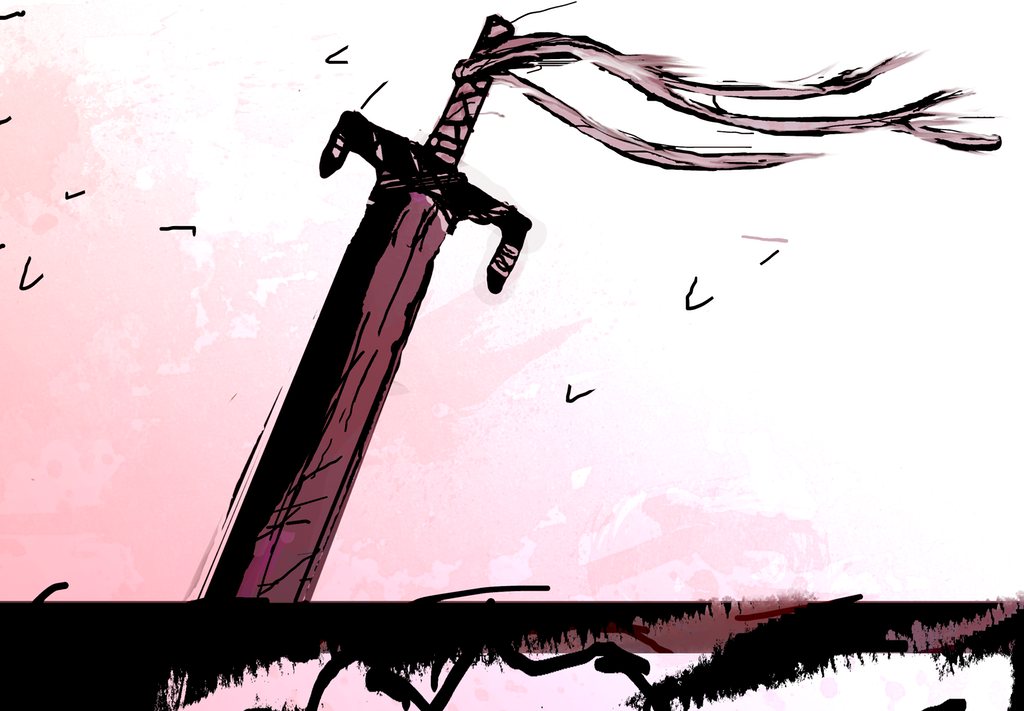
\includegraphics[width=80mm]{./img/otoriagrave.png}
\begin{figure}[h]
\end{figure}
\end{center}

\clearpage
 
 \chapter{Random template shit}
\clearpage






















\begin{figure}[!t]
	\begin{paperbox}{Behold, the Paperbox!}
		The \lstinline!paperbox! is used as a sidebar. It does not break over columns and is best used with a figure environment to float it to one corner of the page where the surrounding text can then flow around it.
	\end{paperbox}
\end{figure}

% For more columns, you can say \begin{dndtable}[your options here].
% For instance, if you wanted three columns, you could say
% \begin{dndtable}[XXX]. The usual host of tabular parameters are
% available as well.
\header{Nice table}
\begin{dndtable}
   	\textbf{Table head}  & \textbf{Table head} \\
   	Some value  & Some value \\
   	Some value  & Some value \\
   	Some value  & Some value
\end{dndtable}

% You can optionally not include the background by saying
% begin{monsterboxnobg}
\begin{monsterbox}{Monster Foo}
  \begin{hangingpar}
    \textit{Small metasyntactic variable (goblinoid), neutral evil}
  \end{hangingpar}
	\hline%
	\basics[%
	armorclass = 12,
	hitpoints  = \dice{3d8 + 3},
	speed      = 50 ft
	]
	\hline%
	\stats[
    STR = \stat{12}, % This stat command will autocomplete the modifier for you
    DEX = \stat{7}
	]
	\hline%
	\details[%
	% If you want to use commas in these sections, enclose the
	% description in braces.
	% I'm so sorry.
	languages = {Common Lisp, Erlang},
	]

	\begin{monsteraction}[Monster-super-powers]
		This Monster has some serious superpowers!
	\end{monsteraction}
	\monstersection{Actions}
	\begin{monsteraction}[Generate text]
		This one can generate tremendous amounts of text! Though only when it wants to.
	\end{monsteraction}

	\begin{monsteraction}[More actions]
    See, here he goes again! Yet more text.
	\end{monsteraction}
\end{monsterbox}

\section{Spells}

\begin{spell}
	{Beautiful Typesetting}
	{4th-level illusion}
	{1 action}
	{5 feet}
	{S, M (ink and parchment, which the spell consumes)}
	{Until dispelled}
	You are able to transform a written message of any length into a beautiful scroll. All creatures within range that can see the scroll must make a wisdom saving throw or be charmed by you until the spell ends.

	While the creature is charmed by you, they cannot take their eyes off the scroll and cannot willingly move away from the scroll. Also, the targets can make a wisdom saving throw at the end of each of their turns. On a success, they are no longer charmed.
\end{spell}

\lipsum[2]

\section{Colors}

This package provides several global color variables to style \lstinline!commentbox!, \lstinline!quotebox!, \lstinline!paperbox!, and \lstinline!dndtable! environments.

\begin{dndtable}[lX]
  \textbf{Color}         & \textbf{Description} \\
  \lstinline!commentboxcolor! & Controls \lstinline!commentbox! background. \\
  \lstinline!paperboxcolor!   & Controls \lstinline!paperbox! background. \\
  \lstinline!quoteboxcolor!   & Controls \lstinline!quotebox! background. \\
  \lstinline!tablecolor!      & Controls background of even \lstinline!dndtable! rows. \\
\end{dndtable}

See Table~\ref{tab:colors} for a list of accent colors that match the core books.

\begin{table*}
  \begin{dndtable}[XX]
    \textbf{Color}                            & \textbf{Description} \\
    \lstinline!PhbLightGreen!                      & Light green used in PHB Part 1 \\
    \lstinline!PhbLightCyan!                       & Light cyan used in PHB Part 2 \\
    \lstinline!PhbMauve!                           & Pale purple used in PHB Part 3 \\
    \lstinline!PhbTan!                             & Light brown used in PHB appendix \\
    \lstinline!DmgLavender!                        & Pale purple used in DMG Part 1 \\
    \lstinline!DmgCoral!                           & Orange-pink used in DMG Part 2 \\
    \lstinline!DmgSlateGray! (\lstinline!DmgSlateGrey!) & Blue-gray used in PHB Part 3 \\
    \lstinline!DmgLilac!                           & Purple-gray used in DMG appendix \\
  \end{dndtable}
  \caption{Colors supported by this package}%
  \label{tab:colors}
\end{table*}

\begin{itemize}
  \item Use \lstinline!\setthemecolor[<color>]! to set \lstinline!themecolor!, \lstinline!commentcolor!, \lstinline!paperboxcolor!, and \lstinline!tablecolor! to a specific color.
  \item Calling \lstinline!\setthemecolor! without an argument sets those colors to the current \lstinline!themecolor!.
  \item \lstinline!commentbox!, \lstinline!dndtable!, \lstinline!paperbox!, and \lstinline!quoteboxcolor! also accept an optional color argument to set the color for a single instance.
\end{itemize}

\subsection{Examples}

\subsubsection{Using \lstinline!themecolor!}

\begin{lstlisting}
\setthemecolor[PhbMauve]

\begin{paperbox}{Example}
  \lipsum[2]
\end{paperbox}

\setthemecolor[PhbLightCyan]

\header{Example}
\begin{dndtable}[cX]
  \textbf{d8} & \textbf{Item} \\
  1           & Small wooden button \\
  2           & Red feather \\
  3           & Human tooth \\
  4           & Vial of green liquid \\
  6           & Tasty biscuit \\
  7           & Broken axe handle \\
  8           & Tarnished silver locket \\
\end{dndtable}
\end{lstlisting}

\begingroup
\setthemecolor[PhbMauve]

\begin{paperbox}{Example}
  \lipsum[2]
\end{paperbox}

\setthemecolor[PhbLightCyan]

\header{Example}
\begin{dndtable}[cX]
  \textbf{d8} & \textbf{Item} \\
  1           & Small wooden button \\
  2           & Red feather \\
  3           & Human tooth \\
  4           & Vial of green liquid \\
  6           & Tasty biscuit \\
  7           & Broken axe handle \\
  8           & Tarnished silver locket \\
\end{dndtable}
\endgroup

\subsubsection{Using element color arguments}

\begin{lstlisting}
\begin{dndtable}[cX][DmgCoral]
  \textbf{d8} & \textbf{Item} \\
  1           & Small wooden button \\
  2           & Red feather \\
  3           & Human tooth \\
  4           & Vial of green liquid \\
  6           & Tasty biscuit \\
  7           & Broken axe handle \\
  8           & Tarnished silver locket \\
\end{dndtable}
\end{lstlisting}

\begin{dndtable}[cX][DmgCoral]
  \textbf{d8} & \textbf{Item} \\
  1           & Small wooden button \\
  2           & Red feather \\
  3           & Human tooth \\
  4           & Vial of green liquid \\
  6           & Tasty biscuit \\
  7           & Broken axe handle \\
  8           & Tarnished silver locket \\
\end{dndtable}

% End document
\end{document}
